% Use the lineno option to display guide line numbers if required.
\documentclass[9pt,twocolumn,twoside,lineno]{pnas-new}

\usepackage{listings}

% Automatic formatting of SI units
\usepackage[binary-units]{siunitx}

% Set options for code listings
\lstset{language=C++}

% Visible TODO notes
\newcommand{\todo}[1]{\textbf{\textsc{\textcolor{red}{(TODO: #1)}}}}

\templatetype{pnasresearcharticle} % Choose template 
% {pnasresearcharticle} = Template for a two-column research article
% {pnasmathematics} %= Template for a one-column mathematics article
% {pnasinvited} %= Template for a PNAS invited submission

\title{Large-scale brain simulations on the desktop using procedural connectivity}

% Use letters for affiliations, numbers to show equal authorship (if applicable) and to indicate the corresponding author
\author[a,1]{James C Knight}
\author[a]{Thomas Nowotny} 

\affil[a]{Centre for Computational Neuroscience and Robotics, School of Engineering and Informatics, University of Sussex, Brighton, United Kingdom}

% Please give the surname of the lead author for the running footer
\leadauthor{Knight} 

% Please add here a significance statement to explain the relevance of your work
\significancestatement{Authors must submit a 120-word maximum statement about the significance of their research paper written at a level understandable to an undergraduate educated scientist outside their field of speciality. The primary goal of the Significance Statement is to explain the relevance of the work in broad context to a broad readership. The Significance Statement appears in the paper itself and is required for all research papers.}

% Please include corresponding author, author contribution and author declaration information
\authorcontributions{J.K. and T.N. wrote the paper.
T.N. is the original developer of GeNN.
J.K. is currently the primary GeNN developer and was responsible for extending the code generation approach to the procedural simulation of synaptic connectivity.
J.K. performed the experiments and the analysis of the results that are presented in this work.}

\authordeclaration{The authors declare no conflict of interest.}
\correspondingauthor{\textsuperscript{1}To whom correspondence should be addressed. E-mail: J.C.Knight\@sussex.ac.uk}

% Keywords are not mandatory, but authors are strongly encouraged to provide them. If provided, please include two to five keywords, separated by the pipe symbol, e.g:
\keywords{spiking neural networks $|$ GPU $|$ high-performance computing $|$ brain simulation} 

\begin{abstract}
Large-scale simulations of spiking neural networks have become important tools in helping us improve our understanding of the dynamics of brain circuits, and ultimately brain function.
However, even small mammals such as mice have on the order of \num{1E12} synaptic connections~\citep{Herculano-Houzel2010} which are typically charaterized by at least one floating point value per synapse, usually related to their synaptic conductance.
If single precision floating point variables were used to store individual conductance values for all synapses of a mouse brain, several terabytes of memory would be required.
Because such memory requirements are beyond what is plausible for a single desktop machine, simulations of large-scale spiking neural networks are currently typically simulated on large distributed high performance computing systems. This is costly and limits this level of modelling to a select few research groups who have access to appropriate supercomputing resources.
However, large parts of current brain models are normally described by means of simple algorithms which determine the connectivity and the strengths of synaptic connections. 
In this work, we describe extensions to GeNN~\citep{Yavuz2016} -- our GPU-based spiking neural network simulator -- that enable it to `procedurally' generate connectivity and synaptic weights 'on the go' as spikes are triggered, rather than generating large connectivity matrices up front and retrieving them from memory when needed, which is how practiaclly all simulations are run today.
We find that high-end GPUs are well-suited to this approach as they provide a large amount of raw computational power which is often under-utilised when simulating spiking neural networks due to the limited memory bandwidth available to each parallel computing element.
To demonstrate the value of this approach, we have implemented a recent model of the Macaque visual cortex consisting of \num{4.13E6} neurons and \num{24.2E9} synapses. With our new method this model can be simulated on a single GPU. We demonstrate that the results match results obtained on a supercomputer and that the simulation runs faster on a singleh high-end GPU than a previous simulation which was executed on over 1000 supercomputer nodes.
\end{abstract}

\dates{This manuscript was compiled on \today}
\doi{\url{www.pnas.org/cgi/doi/10.1073/pnas.XXXXXXXXXX}}

\begin{document}

\maketitle
\thispagestyle{firststyle}
\ifthenelse{\boolean{shortarticle}}{\ifthenelse{\boolean{singlecolumn}}{\abscontentformatted}{\abscontent}}{}

\dropcap{T}he brain of a mouse has around \num{70E6} neurons, but this number is dwarfed by the \num{1E12} synapses which connect them.
%While simulating synaptic plasticity -- the family of mechanisms believed to be %responsible for learning -- represents a further challenge, in a large-scale model, it is unlikely that learning would be enabled on \emph{all} synapses so efficiently simulating the remaining static synapses is a key challenge for large-scale brain simulation.\todo{has this been at all quantified in mice?}
In computer simulations of spiking neural networks, propagating spikes through synapses involves reading a `row' of synapses connecting a spiking presynaptic neuron to its postsynaptic partners and adding the `weight' of each synapse in the row to a `bin' containing the postsynatic neuron's input for the next simulation timestep.
%Because typical EPSP shaping functions are linear, they can then be subsequently applied to the `histogram' resulting from this process.~\todo{presumably someone first had this intuition so cite}.
Typically, the information which neurons are connected by a synapse and with what weight, is generated before a simulation is run and stored in large matrices in random access memories. 
This creates high memory requirements for large-scale brain models, so that they can typically only be simulated on large distributed computer systems using software such as NEST~\citep{Gewaltig2007} or NEURON~\citep{carnevale2006neuron}.
By careful design, these simulators can maintain the memory requirements for each node constant, even when a simulation is distributed across thousands of nodes~\citep{Jordan2018}.
However, high performance computer systems are bulky, expensive and consume large amounts of power, meaning that they are typically shared resources that are only accessible to a limited number of researchers and for strongly time-limited investigations.

Neuromorphic systems~\citep{Frenkel2018,Frenkel2019,Furber2014,Merolla2014,Qiao2015,Schemmel2017} take inspiration from the brain and have been developed specifically as an alternative for simulating large spiking neural networks.
One particular relevant feature of the brain is that its memory elements -- the synapses -- are co-located with the computing elements -- the neurons -- throughout the entire system.
In neuromorphic systems, this often translates to dedicating a large proportion of each chip to memory.
However, while such on-chip memory is fast, it can only be fabricated at relatively low density meaning that many of these systems economize -- either by reducing the maximum number of synapses per neuron to as few as \num{256} or by reducing the precision of the synaptic weights to \num{6}~\citep{Schemmel2017}, \num{4}~\citep{Frenkel2018} or even \SI{1}{\bit}~\citep{Merolla2014,Frenkel2019}.
Such strategies allow some classes of spiking neural networks to be simulated very efficiently, but reducing the degree of connectivity in large-scale brain simulations to fit within the constraints of current neuromorphic systems inevitably changes their dynamics~\citep{VanAlbada2015}.
Unlike the majority of other neuromorphic systems, the SpiNNaker~\citep{Furber2014} neuromorphic super-computer is entirely programmable and combines a large amount of on-chip memory with external memories, distributed across the system for the storage of synaptic connectivity.
SpiNNaker's external memory bandwidth, on-chip memory capacity and the computational power of each core are all tailored to large-scale brain simulation meaning that the output bins of the synapse processing algorithm can fit in on-chip memory and there is enough external memory bandwidth to fetch synaptic rows fast enough for real-time simulation of large-scale models~\citep{Rhodes2019}.
\todo{good argument against SpiNNaker}
This is a promising approach for future research but because of its prototype nature its availability is limited, and a physically large system is still required for even moderately-sized simulations (9 boards for a simulation with around \num{10E3} neurons and \num{300E6} synapses~\citep{Rhodes2019}).
%However, a physically large system is required for even moderately-sized simulations (9 boards for a simulation with around \num{10E3} neurons and \num{300E6} synapses~\citep{Rhodes2019})
%A next generation SpiNNaker system is currently under development~\citep{Mayr2019} and, by employing a newer fabrication technology (\SI{22}{\nano\meter} rather than \SI{130}{\nano\meter}), a single chip of the new system will offer equivalent performance to 48 of the current chips.
%Nonetheless, large-scale brain simulations will still require a large multi-chip system.

Modern GPUs have relatively small amounts of on-chip memory and, instead, dedicate the majority of their silicon area to arithmetic logic units~(ALUs).
GPUs use dedictated hardware to rapidly switch between tasks so that the latency of accessing external memory can be `hidden' behind computation, as long as there is sufficient computation to be performed.
For example, the memory latency of a typical modern GPU can be completely hidden if each CUDA core performs approximately 10 arithmetic operations per byte of data accessed from memory.
Unfortunately, processing a synapse in a spiking neural network simulation is likely to require accessing approximately \SI{8}{\byte} of memory and performing many fewer than the required 80 instructions. This makes synaptic updates highly memory bound.
Nonetheless, we have shown in previous work~\citep{Knight2018} that, as GPUs have significantly higher total memory bandwidth than even the most expensive CPU, moderately sized models of around \num{10E3} neurons and \num{1E9} synapses can be simulated on a single GPU with competitive speed and energy requirements.
Individual GPUs do, however, not have enough memory to simulate truly large-scale brain models and, although small numbers of GPUs can be connected together using the high-speed NVLink~\todo{cite} interconnect, scaling will be dictated by the same communication overheads as for other MPI-based distributed systems beyond such small GPU clusters.

In this work we present a novel approach which converts large-scale brain simulation from a problem which is memory-bound on a GPU to one where the large amount of computational power available on a GPU can be used to reduce both memory and memory bandwidth requirements and enable truly large-scale brain simulations on a single  GPU workstation.

\section*{Results}
In the following we will first two recent innovations in our GeNN simulator~\citep{Yavuz2016} which allow to use it for simulating large-scale models on a single GPU.
We will then demonstrate the power the new features by simulating a recent model of the Macaque visual cortex~\citep{Schmidt2018} consisting of \num{4.13E6} neurons and \num{24.2E9} synapses on a single GPU. We find that we not only obtain the same results as in the previous simulation on a high-performance supercomputer, but our simulation also runs faster.

\subsection*{Procedural connectivity}
Our GeNN simulator~\citep{Yavuz2016} uses code generation to convert neuron and synapse models -- described using `snippets' of C-like code -- into CUDA code for GPU simulation.
We previously extended GeNN to allow the same approach to be applied to generating efficient, parallel model initialisation code from code snippets describing the algorithms to use for initialising individual state variables and synaptic connectivity~\citep{Knight2018}.
Parallelising initialisation in this manner sped up model initialisation by around $20\times$ on a desktop PC, but also indicates just how well-suited these initialisation algorithms are to GPU.
In fact, it seems somewhat illogical to run these algorithms once only to fill the limited memory of the GPU with data and subsequently read it back throughout the simulation 

\begin{figure*}
    \centering
    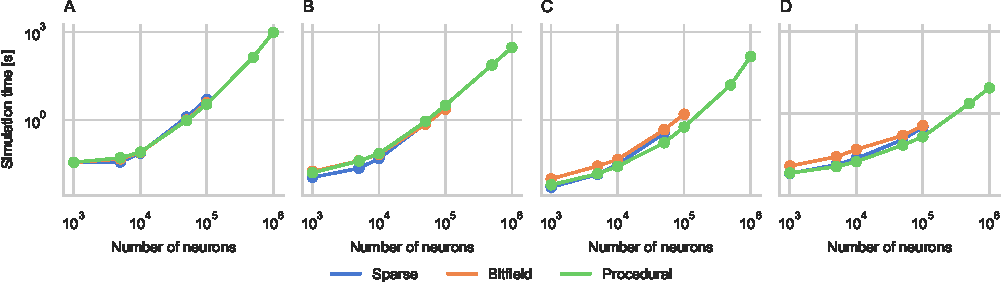
\includegraphics{figures/performance_scaling}
    \caption{Performance scaling on a range of modern GPUs. \textbf{A} The best performing approach at each scale.
    \textbf{B} Raw performance of each approach.}
    \label{fig:performance_scaling}
\end{figure*}

To demonstrate the performance and scalability of this new approach, we ran several simulations of a network, initially designed as a medium for experimentation into signal propagation through cortical networks~\citep{Vogels2005}, but subsequently  widely used as a scalable benchmark~\citep{Brette2007}.
The network consists of \num{10000} integrate-and-fire neurons, split between an excitatory population of \num{8000} cells and an inhibitory population of \num{2000} cells.

\begin{figure*}
    \centering
    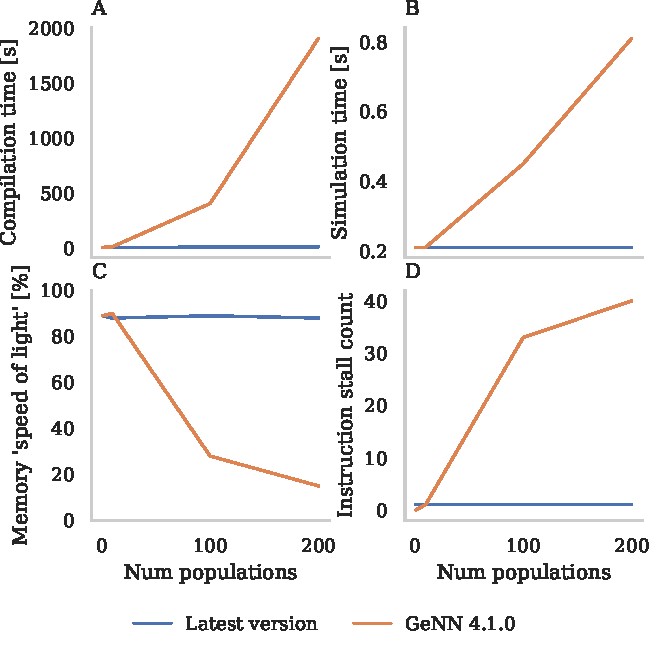
\includegraphics{figures/merging_scaling}
    \caption{Performance of a simulation of \num{1000000} LIF neurons driven by a gaussian input current, partitioned into varying numbers of populations. 
    \textbf{A} Compilation time using GCC 7.5.0.
    \textbf{B} Simulation time for an \SI{1}{\second} simulation.
    \textbf{C} Memory throughput reported by NVIDIA Nsight compute profiler 'Speed of light' metric.
    \textbf{D} Number of 'No instruction' stalls reported by NVIDIA Nsight compute profiler.}
    \label{fig:merging_scaling}
\end{figure*}

\subsection*{Kernel merging}
While the procedural connectivity approach presented in the previous section allows us to simulate models which would otherwise not fit within the memory of a single GPU, there are additional problems when using code generation to generate simulation code for models with large numbers of neuron and synapse populations.

GeNN and -- to the best of our knowledge~\citep{Blundell2018} -- all other SNN simulators which use code generation to generate all of their simulation code (rather than, for example NESTML~\citep{Plotnikov2016}, which uses code generation to generate neuron simulation code) generate seperate pieces of code to simulate each population of neurons and synapses.
This approach allows optimizations such as the hard-coding of constant parameters to be easily performed and, although generating code for models with many populations will result in large code size, C++ CPU code  can be easily divided between multiple modules and compiled in parallel, minimizing the effect on build time.
However, GPUs can only run a small number of kernels -- which are equivalent to modules in this context --  simultaneously (128 on the latest NVIDIA GPUs~\todo{cite}).
Therefore, in GeNN, multiple neuron populations are simulated within each kernel resulting in code such as the following example which illustrates how 3 populations of 1000 neurons could be simulated in a single kernel:

\begin{lstlisting}
void updateNeurons()
{
  if(thread < 1000) {
    // Update neuron population A
  }
  else if(thread >= 1000 && thread < 2000) {
    // Update neuron population B
  }
  else if(thread >= 2000 && thread < 3000) {
    // Update neuron population C
  }
}

\end{lstlisting}

This works well for models with small numbers of populations but, as figure~\ref{fig:merging_scaling}A illustrates, compilation time increases super-linearly with the number of populations (i.e. the size of the neuron kernel) -- quickly becoming impractical.
Additionally, and even more critically, figure~\ref{fig:merging_scaling}B shows that simulations of the same model, artificially divided into more populations, run much slower.
Each thread in this model reads \SI{32}{\byte} of data and, as we discussed previously, hiding the latency of these memory accesses would require approximately 320 arithmetic operations.
Sampling from the uniform distribution and updating a LIF neuron requires many fewer operations than this so we would expect this kernel to be memory bound.
Figure~\ref{fig:merging_scaling}C -- obtained using data from the NVIDIA Nsight compute profiler~\todo{cite} -- shows that this to be true with the memory system being around \SI{90}{\percent} utilised for small numbers of populations.
However, if the model is partitioned into large numbers of populations, the kernel stops being able to efficiently use the memory.
Investigating the performance counters

\begin{lstlisting}
struct NeuronUpdateGroup
{
  unsigned int numNeurons;
  float* V; 
};

NeuronUpdateGroup neuronUpdateGroup
{
  {1000, d_VA},
  {1000, d_VB},
  {1000, d_VC}
};

void updateNeurons()
{
  if(thread < 3000) {
    // Determine which population thread
    // should be processing and update using 
    // variables in neuronUpdateGroup
  }
}
\end{lstlisting}

\begin{figure*}
    \centering
    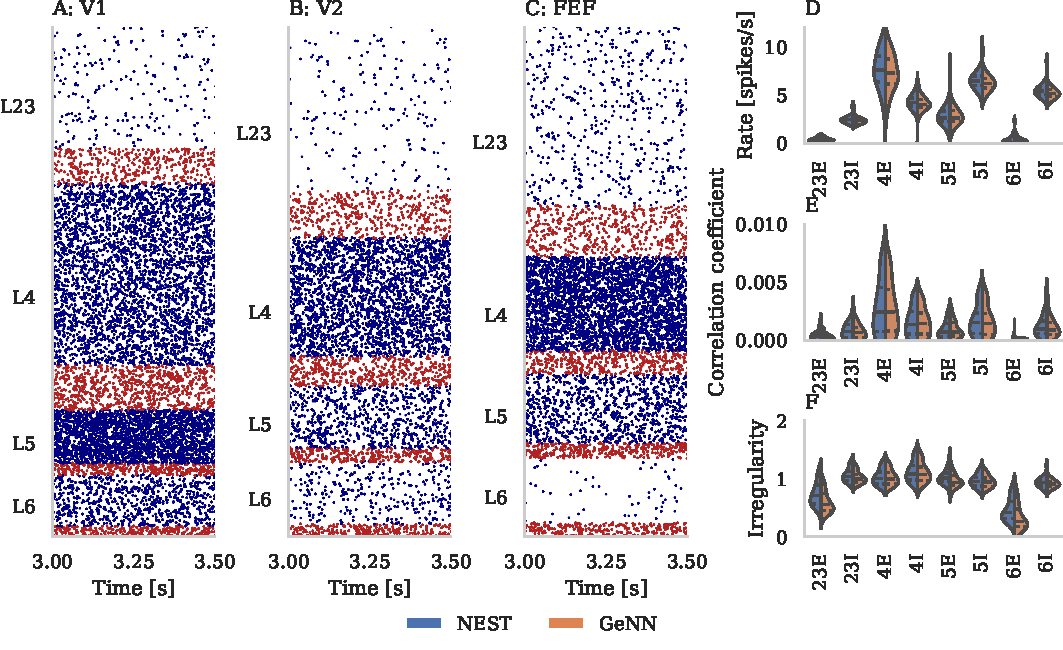
\includegraphics{figures/multi_area}
    \caption{Results of full-scale multi-area model simulation. 
    \textbf{A-C} Raster plots of spiking activity of \SI{3}{\percent} of the neurons in area V1~\textbf{A}, V2~\textbf{B}, and FEF~\textbf{C}. 
    Blue: excitatory neurons, red: inhibitory neurons.
    \textbf{D-F} Spiking statistics for each population across all 32 areas simulated using GeNN and NEST shown as split violin plots.
    Solid lines: medians, Dashed lines: Interquartile range~(IQR).
    \textbf{D} Population-averaged firing rates.
    \textbf{E} Average pairwise correlation coefficients ofspiking activity. 
    \textbf{F} Irregularity measured by revised local variation LvR~\citep{Shinomoto2009} averaged across neurons.}
    \label{fig:multi_area}
\end{figure*}

\subsection*{The multi-area model}
Due to lack of computing power and sufficiently detailed connectivity data, previous models of the cortex have either focussed on modelling individual local microcircuits~\citep{Izhikevich2008,Potjans2012} at the level of individual cells or modelling multiple connected areas at a higher level of abstraction where entire ensembles of neurons are described by a small number of differential equations~\todo{find citation}.
However, data from several species~\todo{find citation} has shown that cortical activity has distinct features at both the global and local levels which can be captured by modelling interconnected microcircuits at the level of individual cells.

By using a supercomputer to simulate a model based on the latest connectivity data and The multi-scale model of the macaque visual cortex~\citep{Schmidt2018} developed by 

\section*{Discussion}
\begin{itemize}
    \item Further scaling - memory only required for neuron parameters
    \item Learning
    \item Hardware for procedural connectivity?
\end{itemize}
% 
% \section*{Guide to using this template on Overleaf}
% 
% Please note that whilst this template provides a preview of the typeset manuscript for submission, to help in this preparation, it will not necessarily be the final publication layout. For more detailed information please see the \href{http://www.pnas.org/site/authors/format.xhtml}{PNAS Information for Authors}.
% 
% If you have a question while using this template on Overleaf, please use the help menu (``?'') on the top bar to search for \href{https://www.overleaf.com/help}{help and tutorials}. You can also \href{https://www.overleaf.com/contact}{contact the Overleaf support team} at any time with specific questions about your manuscript or feedback on the template.
% 
% \subsection*{Author Affiliations}
% 
% Include department, institution, and complete address, with the ZIP/postal code, for each author. Use lower case letters to match authors with institutions, as shown in the example. Authors with an ORCID ID may supply this information at submission.
% 
% \subsection*{Submitting Manuscripts}
% 
% All authors must submit their articles at \href{http://www.pnascentral.org/cgi-bin/main.plex}{PNAScentral}. If you are using Overleaf to write your article, you can use the ``Submit to PNAS'' option in the top bar of the editor window. 
% 
% \subsection*{Format}
% 
% Many authors find it useful to organize their manuscripts with the following order of sections;  Title, Author Affiliation, Keywords, Abstract, Significance Statement, Results, Discussion, Materials and methods, Acknowledgments, and References. Other orders and headings are permitted.
% 
% \subsection*{Manuscript Length}
% 
% PNAS generally uses a two-column format averaging 67 characters, including spaces, per line. The maximum length of a Direct Submission research article is six pages and a Direct Submission Plus research article is ten pages including all text, spaces, and the number of characters displaced by figures, tables, and equations.  When submitting tables, figures, and/or equations in addition to text, keep the text for your manuscript under 39,000 characters (including spaces) for Direct Submissions and 72,000 characters (including spaces) for Direct Submission Plus.
% 
% \subsection*{References}
% 
% References should be cited in numerical order as they appear in text; this will be done automatically via bibtex, e.g. \cite{belkin2002using} and \cite{berard1994embedding,coifman2005geometric}. All references should be included in the main manuscript file.  
% 
% \subsection*{Data Archival}
% 
% PNAS must be able to archive the data essential to a published article. Where such archiving is not possible, deposition of data in public databases, such as GenBank, ArrayExpress, Protein Data Bank, Unidata, and others outlined in the Information for Authors, is acceptable.
% 
% \subsection*{Language-Editing Services}
% Prior to submission, authors who believe their manuscripts would benefit from professional editing are encouraged to use a language-editing service (see list at www.pnas.org/site/authors/language-editing.xhtml). PNAS does not take responsibility for or endorse these services, and their use has no bearing on acceptance of a manuscript for publication. 
% 
% \begin{figure}%[tbhp]
%     \centering
%     
\includegraphics[width=.8\linewidth]{frog}
%     \caption{Placeholder image of a frog with a long example caption to show justification setting.}
%     \label{fig:frog}
% \end{figure}
% 
% 
% \begin{SCfigure*}[\sidecaptionrelwidth][t]
%     \centering
%     
\includegraphics[width=11.4cm,height=11.4cm]{frog}
%     \caption{This caption would be placed at the side of the figure, rather than below it.}\label{fig:side}
% \end{SCfigure*}
% 
% \subsection*{Digital Figures}
% 
% Only TIFF, EPS, and high-resolution PDF for Mac or PC are allowed for figures that will appear in the main text, and images must be final size. Authors may submit U3D or PRC files for 3D images; these must be accompanied by 2D representations in TIFF, EPS, or high-resolution PDF format.  Color images must be in RGB (red, green, blue) mode. Include the font files for any text. 
% 
% Figures and Tables should be labelled and referenced in the standard way using the \verb|\label{}| and \verb|\ref{}| commands.
% 
% Figure \ref{fig:frog} shows an example of how to insert a column-wide figure. To insert a figure wider than one column, please use the \verb|\begin{figure*}...\end{figure*}| environment. Figures wider than one column should be sized to 11.4 cm or 17.8 cm wide. Use \verb|\begin{SCfigure*}...\end{SCfigure*}| for a wide figure with side captions.
% 
% \subsection*{Tables}
% In addition to including your tables within this manuscript file, PNAS requires that each table be uploaded to the submission separately as a “Table” file.  Please ensure that each table .tex file contains a preamble, the \verb|\begin{document}| command, and the \verb|\end{document}| command. This is necessary so that the submission system can convert each file to PDF.
% 
% \subsection*{Single column equations}
% 
% Authors may use 1- or 2-column equations in their article, according to their preference.
% 
% To allow an equation to span both columns, use the \verb|\begin{figure*}...\end{figure*}| environment mentioned above for figures.
% 
% Note that the use of the \verb|widetext| environment for equations is not recommended, and should not be used. 
% 
% \begin{figure*}[bt!]
%     \begin{align*}
%         (x+y)^3&=(x+y)(x+y)^2\\
%             &=(x+y)(x^2+2xy+y^2) \numberthis \label{eqn:example} \\
%             &=x^3+3x^2y+3xy^3+x^3. 
%     \end{align*}
% \end{figure*}
% 
% 
% \begin{table}%[tbhp]
%     \centering
%     \caption{Comparison of the fitted potential energy surfaces and ab initio benchmark electronic energy calculations}
%     \begin{tabular}{lrrr}
%         Species & CBS & CV & G3 \\
%         \midrule
%         1. Acetaldehyde & 0.0 & 0.0 & 0.0 \\
%         2. Vinyl alcohol & 9.1 & 9.6 & 13.5 \\
%         3. Hydroxyethylidene & 50.8 & 51.2 & 54.0\\
%         \bottomrule
%     \end{tabular}
% 
%     \addtabletext{nomenclature for the TSs refers to the numbered species in the table.}
% \end{table}
% 
% \subsection*{Supporting Information (SI)}
% 
% Authors should submit SI as a single separate PDF file, combining all text, figures, tables, movie legends, and SI references.  PNAS will publish SI uncomposed, as the authors have provided it.  Additional details can be found here: \href{http://www.pnas.org/page/authors/journal-policies}{policy on SI}.  For SI formatting instructions click \href{https://www.pnascentral.org/cgi-bin/main.plex?form_type=display_auth_si_instructions}{here}.  The PNAS Overleaf SI template can be found \href{https://www.overleaf.com/latex/templates/pnas-template-for-supplementary-information/wqfsfqwyjtsd}{here}.  Refer to the SI Appendix in the manuscript at an appropriate point in the text. Number supporting figures and tables starting with S1, S2, etc.
% 
% Authors who place detailed materials and methods in an SI Appendix must provide sufficient detail in the main text methods to enable a reader to follow the logic of the procedures and results and also must reference the SI methods. If a paper is fundamentally a study of a new method or technique, then the methods must be described completely in the main text.
% 
% \subsubsection*{SI Datasets} 
% 
% Supply Excel (.xls), RTF, or PDF files. This file type will be published in raw format and will not be edited or composed.
% 
% 
% \subsubsection*{SI Movies}
% 
% Supply Audio Video Interleave (avi), Quicktime (mov), Windows Media (wmv), animated GIF (gif), or MPEG files and submit a brief legend for each movie in a Word or RTF file. All movies should be submitted at the desired reproduction size and length. Movies should be no more than 10 MB in size.
% 
% 
% \subsubsection*{3D Figures}
% 
% Supply a composable U3D or PRC file so that it may be edited and composed. Authors may submit a PDF file but please note it will be published in raw format and will not be edited or composed.


\matmethods{Please describe your materials and methods here. This can be more than one paragraph, and may contain subsections and equations as required. Authors should include a statement in the methods section describing how readers will be able to access the data in the paper. 
\begin{itemize}
    \item LIF neuron
    \item Exponential static synapses
    \item Connectivity
    \item Parameter values for scaling and merging experiments
\end{itemize}
\subsection*{Neuron models}
Example text for subsection.
}

\showmatmethods{} % Display the Materials and Methods section

\acknow{Please include your acknowledgments here, set in a single paragraph. Please do not include any acknowledgments in the Supporting Information, or anywhere else in the manuscript.}

\showacknow{} % Display the acknowledgments section

% Bibliography
\bibliography{procedural}

\end{document}
